%%%%%%%%%%%%%%%%%%%%%%%%%%%%%%%%%%%%%%%%%%%%%%%%%%%%%%%%%%%%%%%%%%%%%%
%%%%%%%%%%%%%%%%%%%%%%%%%%%%%%%%%%%%%%%%%%%%%%%%%%%%%%%%%%%%%%%%%%%%%%
%% Type of document:
%% - Paperformat: letterpaper, a4paper, a5paper, b5paper,
%%   executivepaper, legalpaper
%% - Main font size: 10pt, 11pt, 12pt
%% - Formulae setting: - (centred), fleqn (left-aligned)
%% - Numbering of formulae: - (right-aligned), leqno (left-aligned)
%% - New page after title: titlepage, notitlepage
%% - Number of columns per page: onecolumn, twocolumn
%% - Page style: oneside, twoside
%% - Paper rotation: - (protrait), landscape
%% - Chapter start: openright, openany
%% - Mark overfull boxes: draft, final
\documentclass[a4paper,11pt,fleqn,titlepage,onecolumn,twoside,openany,final]{report}
%%%%%%%%%%%%%%%%%%%%%%%%%%%%%%%%%%%%%%%%%%%%%%%%%%%%%%%%%%%%%%%%%%%%%%
%% borders, margrins and offset
\usepackage[a4paper,left=1.0in,right=1.0in,top=0.5in,bottom=0.5in,includeheadfoot]{geometry}
%%\openup-2pt
%%%%%%%%%%%%%%%%%%%%%%%%%%%%%%%%%%%%%%%%%%%%
%%%%%%%%%%%%%%%%%%%%%%%%%%%%%%%%%%%%%%%%%%%%
%%\usepackage[sf,bf]{titlesec}
\usepackage[compact,sf,bf]{titlesec}

% def of subpart begin
% !! DOES NOT WORK !!
%%\usepackage{tocloft}
\usepackage{lipsum}
\usepackage{fmtcount}
\newcommand\subpartname{Subpart}
\titleclass{\subpart}{top}[\part]
\newcounter{subpart}
\renewcommand\thesubpart{\Numberstring{subpart}}

\makeatletter
\titleformat%
{\subpart}[display]%
{\normalsize\Huge\filcenter}% font
{\scshape\subpartname~\thesubpart}% numbering
{1em}%
{}
%{{\bfseries#1}\iftitlemeasuring{\def\ttl@endlongest{\clearpage}}{}}
%above line was in example from stackexchange, but did not compile. 
%replaced it therefore with an empty command; don't know what this
%omits now. kai, dec'15

\titlespacing*{\subpart}{0pt}{0em}{\pagetotal}

\makeatother

\newcommand\subpartautorefname{\subpartname}
\newcommand\subpartbreak{\cleardoublepage\mbox{}\vfil}

\assignpagestyle{\subpart}{plain}

\makeatletter
\newcommand*\l@subpart[2]{%
  \ifnum \c@tocdepth >-2\relax
    \addpenalty{-\@highpenalty}%
    \addvspace{1em \@plus\p@}%
    \setlength\@tempdima{3.5em}%
    \begingroup
      \parindent \z@ \rightskip \@pnumwidth
      \parfillskip -\@pnumwidth
      {\leavevmode
       \large\subpartname~#1\hfil\hb@xt@\@pnumwidth{\hss #2}}\par
       \nobreak
         \global\@nobreaktrue
         \everypar{\global\@nobreakfalse\everypar{}}%
    \endgroup
  \fi}
\makeatother
% def of subpart end


%%%%%%%%%%%%%%%%%%%%%%%%%%%%%%%%%%%%%%%%%%%%
%%%%%%%%%%%%%%%%%%%%%%%%%%%%%%%%%%%%%%%%%%%%%%%%%%%%%%%%%%%%%%%%%%%%%%
%% providing if-then-else command:
\usepackage{ifthen}
%%%%%%%%%%%%%%%%%%%%%%%%%%%%%%%%%%%%%%%%%%%%%%%%%%%%%%%%%%%%%%%%%%%%%%
\usepackage[english]{babel}%
%%%%%%%%%%%%%%%%%%%%%%%%%%%%%%%%%%%%%%%%%%%%%%%%%%%%%%%%%%%%%%%%%%%%%%
%% Header and footer definition:
\usepackage{fancyhdr}%

%\fancypagestyle{plain}{%
%\fancyhf{} % clear all header and footer fields 
%\fancyfoot[RO, LE]{\footnotesize \thepage} % except the center
%\renewcommand{\headrulewidth}{0pt}
%\renewcommand{\footrulewidth}{0pt}}

\pagestyle{fancy}%
\fancyhf{}%
\fancyhead[RO]{\slshape \footnotesize \nouppercase{\rightmark}}
\fancyhead[LE]{\slshape \footnotesize \nouppercase{\leftmark}}


%\fancyhead[R]{\slshape \footnotesize \nouppercase{\myyear}}%
%\fancyhead[L]{\slshape \footnotesize \nouppercase{\mytitle}}%
\fancyfoot[RO, LE]{\footnotesize \thepage}%
\renewcommand{\headrulewidth}{0.5pt}%
\renewcommand{\footrulewidth}{0pt}%

\fancypagestyle{plainstyle}
{
   \fancyhf{}
   \fancyfoot{}
	 \renewcommand{\headrulewidth}{0pt}%
}

%%%%%%%%%%%%%%%%%%%%%%%%%%%%%%%%%%%%%%%%%%%%%%%%%%%%%%%%%%%%%%%%%%%%%%
%% paragraph settings:
\setlength{\parindent}{0in}%
\setlength{\parskip}{10pt}
%%\setlength{\parindent}{.2in}%
%%\setlength{\parskip}{0pt}
%%%%%%%%%%%%%%%%%%%%%%%%%%%%%%%%%%%%%%%%%%%%%%%%%%%%%%%%%%%%%%%%%%%%%%
%% caption settings:
\usepackage[nooneline,format=hang]{caption}
%%%%%%%%%%%%%%%%%%%%%%%%%%%%%%%%%%%%%%%%%%%%%%%%%%%%%%%%%%%%%%%%%%%%%%
%% Define the depth of numbering parts,chapter,sections and paragraphs:
%%   Numbers representing the depth of sectional units:
%%   -1 = \part    (in book or report document classes)
%%    0 = \chapter (in book or report document classes)
%%    0 = \part    (in article document classes)
%%    1 = \section
%%    2 = \subsection
%%    3 = \subsubsection
%%    4 = \paragraph
%%    5 = \subparagraph
\setcounter{secnumdepth}{3}
%%%%%%%%%%%%%%%%%%%%%%%%%%%%%%%%%%%%%%%%%%%%%%%%%%%%%%%%%%%%%%%%%%%%%%
%% citation style:
\usepackage[round,sectionbib]{natbib}
\usepackage{chapterbib}

\newcommand{\bibpc}{{
\footnotesize
\parskip0pt
\setlength{\bibsep}{0.2em}
\bibliographystyle{0/template_ivt-eng}
\bibliography{0/added_bibs,0/ivt_bibs,0/tub,0/ref-gunnar,0/michalm_matsim_book,0/laemmel}
\normalsize
}
}% bibliography per chapter

%%%%%%%%%%%%%%%%%%%%%%%%%%%%%%%%%%%%%%%%%%%%%%%%%%%%%%%%%%%%%%%%%%%%%%
\usepackage{ifthen}

%%%%%%%%%%%%%%%%%%%%%%%%%%%%%%%%%%%%%%%%%%%%%%%%%%%%%%%%%%%%%%%%%%%%%%
\usepackage[usenames,dvipsnames]{xcolor}
\usepackage{xargs}
\usepackage[colorinlistoftodos,prependcaption,textsize=footnotesize]{todonotes}

\newcommandx{\atend}[2][1=]{\todo[linecolor=yellow,backgroundcolor=yellow!25,bordercolor=yellow,#1]{at end: #2}}
\newcommandx{\kaitodo}[2][1=]{\todo[linecolor=red,backgroundcolor=red!25,bordercolor=red,#1]{kai: #2}}
\let\todokai=\kaitodo
\newcommandx{\ahtodo}[2][1=]{\todo[linecolor=blue,backgroundcolor=blue!25,bordercolor=blue,#1]{ah: #2}}
\let\todoah=\ahtodo
\newcommandx{\someonetodo}[2][1=]{\todo[linecolor=yellow,backgroundcolor=yellow!25,bordercolor=yellow,#1]{someone: #2}}
\let\todosomeone=\someonetodo
\newcommandx{\bktodo}[2][1=]{\todo[linecolor=OliveGreen,backgroundcolor=OliveGreen!25,bordercolor=OliveGreen,#1]{bk: #2}}

%%%%%%%%%%%%%%%%%%%%%%%%%%%%%%%%%%%%%%%%%%%%%%%%%%%%%%%%%%%%%%%%%%%%%%
%% Font:
\usepackage{times}
%%%%%%%%%%%%%%%%%%%%%%%%%%%%%%%%%%%%%%%%%%%%%%%%%%%%%%%%%%%%%%%%%%%%%%
%% To prevent overfull boxes
%%   it is quite nice, but in special cases, you will have too large
%%   speaces between a two words of the same line.
\sloppy
%%%%%%%%%%%%%%%%%%%%%%%%%%%%%%%%%%%%%%%%%%%%%%%%%%%%%%%%%%%%%%%%%%%%%%
%% providing umlauts:
%\usepackage[latin1]{inputenc}
%\usepackage[T1]{fontenc}
%%\usepackage[utf8]{inputenc}
\usepackage{ifxetex}
\ifxetex
  \usepackage{fontspec}
  \usepackage{xunicode}
  \usepackage{xltxtra}
\else
  \usepackage[utf8]{inputenc}
\fi
%%%%%%%%%%%%%%%%%%%%%%%%%%%%%%%%%%%%%%%%%%%%%%%%%%%%%%%%%%%%%%%%%%%%%%
%%%%%%%%%%%%%%%%%%%%%%%%%%%%%%%%%%%%%%%%%%%%%%%%%%%%%%%%%%%%%%%%%%%%%%
%% line spacing
\usepackage{setspace}
\onehalfspacing
%%%%%%%%%%%%%%%%%%%%%%%%%%%%%%%%%%%%%%%%%%%%%%%%%%%%%%%%%%%%%%%%%%%%%%
%% letter spacing [[?????]]
\usepackage{soul}
%%\usepackage{ulem}
%%%%%%%%%%%%%%%%%%%%%%%%%%%%%%%%%%%%%%%%%%%%%%%%%%%%%%%%%%%%%%%%%%%%%%
%% no indentation for formulas:
\usepackage[fleqn]{amsmath}
\setlength\mathindent{0pt}
%%%%%%%%%%%%%%%%%%%%%%%%%%%%%%%%%%%%%%%%%%%%%%%%%%%%%%%%%%%%%%%%%%%%%%
%% providing graphics:
\usepackage{graphics}
\usepackage{graphicx}
%%%%%%%%%%%%%%%%%%%%%%%%%%%%%%%%%%%%%%%%%%%%%%%%%%%%%%%%%%%%%%%%%%%%%%
%% sideways figures and tables:
\usepackage{rotating}
%%%%%%%%%%%%%%%%%%%%%%%%%%%%%%%%%%%%%%%%%%%%%%%%%%%%%%%%%%%%%%%%%%%%%%
%% sub-figures:
\usepackage[FIGTOPCAP]{subfigure}
\def\subfigtopskip{0pt}
\def\subfigbottomskip{5pt}
\def\subfigcapskip{0pt}
%%%%%%%%%%%%%%%%%%%%%%%%%%%%%%%%%%%%%%%%%%%%%%%%%%%%%%%%%%%%%%%%%%%%%%
%% figures:
%%   The following are sometimes needed to avoid pushing
%%   the figs to the end of the text.
\def\textfraction{0.0}
\def\topfraction{0.9999}
\def\floatpagefraction{0.9}
%%%%%%%%%%%%%%%%%%%%%%%%%%%%%%%%%%%%%%%%%%%%%%%%%%%%%%%%%%%%%%%%%%%%%%
%% tables:
\usepackage{tabularx}
\usepackage{multirow}
%%%%%%%%%%%%%%%%%%%%%%%%%%%%%%%%%%%%%%%%%%%%%%%%%%%%%%%%%%%%%%%%%%%%%%
\usepackage{hyphenat} % for \hyp support
\usepackage{fixltx2e} % for \textsubscript{...}
\usepackage{booktabs}	% for \toprule. \midrule, \bottomrule in tables
\usepackage{verbatim}
\usepackage{amssymb}	% for \checkmark
\usepackage{amsmath}
\usepackage{pifont}	% for \xmark and \xmark
\newcommand{\cmark}{\ding{51}}% another checkmark symbol
\newcommand{\xmark}{\ding{55}}% an xmark symbol

\usepackage{tikz} % for diagonal line in tables
\usepackage{afterpage} % for  \afterpage{\clearpage}
\usepackage{paralist}	% for compactitems
\usepackage{multicol}
\usepackage{longtable}
\usepackage[stable]{footmisc}
\usepackage{algorithmic}
\usepackage{color}
\usepackage{marvosym}
\usepackage{verbatim}
\usepackage{rotating}
\usepackage[section]{placeins}
\usepackage{eurosym}
\usepackage{bookmark,hyperref}
\usepackage{matsimbook}
\usepackage{framed}
\usepackage{array}
\usepackage{wrapfig}

\usepackage{makeidx}
\makeindex

% make gls entries in the following format ``acr (long desc)''
\AtBeginDocument{%
  \defglsdisplayfirst[\acronymtype]{%
    \glsentryshort{\glslabel} (\glsentrylong{\glslabel})#4%
  }%
}

%\usepackage[toc]{glossaries}
\usepackage[]{glossaries}
\renewcommand*{\acronymtype}{acronym}
\newglossary[alg]{acronym}{acr}{acn}{Acronyms}
\makeglossaries

% \acrfull{...} does not work any more as a result of the above when it is the first occurence of the label; it produces something like ``<abr> (<full>) (<abr> (<full>))''. 
% One can instead use \glsunset{<label>)\acrfull{<label>}

\usepackage{csquotes}
%%%%%%%%%%%%%%%%%%%%%%%%%%%%%%%%%%%%%%%%%%%%%%%%%%%%%%%%%%%%%%%%%%%%%%
%% convenient referencing:
\usepackage[capitalize]{cleveref}
%%%%%%%%%%%%%%%%%%%%%%%%%%%%%%%%%%%%%%%%%%%%%%%%%%%%%%%%%%%%%%%%%%%%%%
%% make definition of abbreviations easier
\usepackage{xspace}
%%%%%%%%%%%%%%%%%%%%%%%%%%%%%%%%%%%%%%%%%%%%%%%%%%%%%%%%%%%%%%%%%%%%%%
%% allows to use full-page background pictures, e.g. for part-titles
\usepackage{wallpaper}
%%%%%%%%%%%%%%%%%%%%%%%%%%%%%%%%%%%%%%%%%%%%%%%%%%%%%%%%%%%%%%%%%%%%%%
%% alternative to paralist
\newcommand{\styleEnumerate}{%
	%\setlength{\itemsep}{-\parskip}%
	%\setlength{\topsep}{-5pt}%
}
\newcommand{\styleItemize}{%
	\styleEnumerate%
	% at the moment, this does not differ from the enumeration-style
}
\newcommand{\styleDescription}{%
	\styleEnumerate%
	% at the moment, this does not differ from the enumeration-style
}

\usepackage{enumitem}
\setlist{itemsep=4pt, topsep=0pt, parsep=4pt, partopsep=0pt}
% I changed parsep to same as itemsep.  I find this easier to read, and I think that it looks cleaner.  If not ok, pls change back.  Kai, aug'15

%%%%%%%%%%%%%%%%%%%%%%%%%%%%%%%%%%%%%%%%%%%%%%%%%%%%%%%%%%%%%%%%%%%%%%
% BDI:
\usepackage{tikz,pgf,pgfplots}
\usetikzlibrary{arrows,decorations,backgrounds,matrix,automata,
trees,shapes,shadows,plotmarks,calc,positioning,patterns,chains,fit}

\usepackage{epsfig}
\usepackage{pdfpages}
\usepackage{tablefootnote}

\newcounter{bean}

\newenvironment{tightenumerate}{
                \begin{list}{
                  {\mbox {
                      \arabic{bean}.\/}}}{\usecounter{bean}
                      \setlength{\itemsep}{-1pt}\setlength{\topsep}{0pt}}}{
                \end{list}}

\newenvironment{tightitemize}{
                \begin{list}{$\bullet$}{
                    \setlength{\itemsep}{-1pt}}{\setlength{\topsep}{0pt}}}{
                \end{list}}
								
\newcommand{\Omit}[1]{}

%%%%%%%%%%%%%%%%%%%%%%%%%%%%%%%%%%%%%%%%%%%%%%%%%%%%%%%%%%%%%%%%%%%%%%
%% pretty printing:
\usepackage{listings}
%%%%%%%%%%%%%%%%%%%%%%%%%%%%%%%%%%%%%%%%%%%%%%%%%%%%%%%%%%%%%%%%%%%%%%
%% XML code setup:
% not used; use \begin{xml} instead. kai, apr'15
%%\lstloadlanguages{XML}
%%%%
%%\lstset {
%%  belowskip=-4pt,
%%  showstringspaces=false,
%%  basicstyle=\ttfamily\footnotesize,
%%  lineskip=0pt,
%%  breaklines=true,
%%  breakatwhitespace=true,
%%  breakindent=12pt,
%%  fontadjust=true,
%%  keywordstyle=\bfseries,
%%  commentstyle=\bfseries,
%%  stringstyle=\bfseries,
%%  xleftmargin=0mm,
%%  xrightmargin=0mm,
%%  tabsize=2
%%}
%%%%%%%%%%%%%%%%%%%%%%%%%%%%%%%%%%%%%%%%%%%%%%%%%%%%%%%%%%%%%%%%%%%%%%
%%
%% The following defines language specific words
%%   These are internal commands. They are not used in the main file.
%%   Langugage specific word commands always starts with '\word'
%%
%% Quelle/Source
\newcommand{\wordsource}{\iflanguage{english}{Source:\ }{\iflanguage{german}{Quelle:\ }{\langerrmessage}}}
%%%%%%%%%%%%%%%%%%%%%%%%%%%%%%%%%%%%%%%%%%%%%%%%%%%%%%%%%%%%%%%%%%%%%%

%%%%%%%%%%%%%%%%%%%%%%%%%%%%%%%%%%%%%%%%%%%%%%%%%%%%%%%%%%%%%%%%%%%%%%
%% \internmakethreecolumns{entry1}{entry2}{entry3}
%%   creates a table with three columns containing the given entries
\newcommand{\internmakethreecolumns}[3]{
  \noindent
  \begin{tabular*}{\textwidth}{@{}l@{}l@{}l@{}}
    #1 & #2 & #3 \\
  \end{tabular*}
}

%%%%%%%%%%%%%%%%%%%%%%%%%%%%%%%%%%%%%%%%%%%%%%%%%%%%%%%%%%%%%%%%%%%%%%
%% Figure definition
%%   \createfigure[<pos>]
%%     {<short caption>}
%%     {<long caption>}
%%     {<\label{label}>}
%%     {<\includegraphics[...]{figure}>}
%%     {<source>or<>}
\newcommand{\createfigure}[6][htp]{%
\begin{figure}[#1] % do not indent this line; produces unwanted spaces.  kai, dec'14
    \caption[#2]{#3.} #4
    \vspace{0.5em}
    \hrule
    \begin{center}
      #5\\
    \end{center}
    \ifthenelse
      {\equal{#6}{}}
      {}
      {\wordsource #6 \vspace{0.5em}}
    \hrule
  \end{figure}%
}
% The syntax "[6][htp]{...[#1]..." means that the first parameter is
% optional. kai, dec'14 
%
% Kommentar Kai: Mir macht diese private
% Definition einige Probleme, weil mein emacs syntax-parser (der
% z.B. bei den Querverweisen hilft), damit natürlich nicht zurecht
% kommt. :-(
%%%%%%%%%%%%%%%%%%%%%%%%%%%%%%%%%%%%%%%%%%%%%%%%%%%%%%%%%%%%%%%%%%%%%%
%% Sideways figure definition
%%   \createfigure
%%     {<short caption>}
%%     {<long caption>}
%%     {<\label{label}>}
%%     {<\includegraphics[...]{figure}>}
%%     {<source>or<>}
\newcommand{\createsidewaysfigure}[5]{
  \begin{sidewaysfigure}
    \caption[#1]{#2.} #3
    \vspace{0.5em}
    \hrule
    \begin{center}
      #4\\
    \end{center}
    \ifthenelse
      {\equal{#5}{}}
      {}
      {\wordsource #5 \vspace{0.5em}}
    \hrule
  \end{sidewaysfigure}
}
%%%%%%%%%%%%%%%%%%%%%%%%%%%%%%%%%%%%%%%%%%%%%%%%%%%%%%%%%%%%%%%%%%%%%%
%% Sub-figure:
%%   \createsubfigure
%%     {<caption>}
%%     {<\includegraphics[...]{figure}>}
%%     {<\label{label}>}
%%     {<\\>or<>}%
\newcommand{\createsubfigure}[4]{
  \subfigure[#1.]{%
    #2%
    #3%
  }#4
}
%%%%%%%%%%%%%%%%%%%%%%%%%%%%%%%%%%%%%%%%%%%%%%%%%%%%%%%%%%%%%%%%%%%%%%
%% Table:
%%   \createtable
%%     {<short caption>}
%%     {<long caption>}
%%     {<\label{label}>}
%%     {<\begin{tabular}...\end{tabular}>}
%%     {<source>or<>}
\newcommand{\createtable}[6][htp]{
  \begin{table}[#1]
    \caption[#2]{#3.} #4
    \vspace{0.5em}
    \hrule
    \begin{center}
      #5\\
    \end{center}
    \ifthenelse
      {\equal{#6}{}}
      {}
      {\wordsource #6 \vspace{0.5em}}
    \hrule
  \end{table}
}
%%%%%%%%%%%%%%%%%%%%%%%%%%%%%%%%%%%%%%%%%%%%%%%%%%%%%%%%%%%%%%%%%%%%%%
%% Sideways table definition
%%   \createsidewaystable
%%     {<short caption>}
%%     {<long caption>}
%%     {<\label{label}>}
%%     {<\begin{tabular}...\end{tabular}>}
%%     {<source>or<>}
\newcommand{\createsidewaystable}[5]{
  \begin{sidewaystable}
    \caption[#1]{#2} #3
    \vspace{0.5em}
    \hrule
    \begin{center}
      #4\\
    \end{center}
    \ifthenelse
      {\equal{#5}{}}
      {}
      {\wordsource #5 \vspace{0.5em}}
    \hrule
  \end{sidewaystable}
}
%%%%%%%%%%%%%%%%%%%%%%%%%%%%%%%%%%%%%%%%%%%%%%%%%%%%%%%%%%%%%%%%%%%%%%
%% XML-figure
%%   \createxmlfigure
%%     {<short caption>}
%%     {<long caption>}
%%     {<\label{label}>}
%%     {<the/file/with/the/xml/code/to/include>}
%%     {<source>or<>}
\newcommand{\createxmlfigure}[5]{
  \begin{figure}
    \caption[#1]{\kai{if this is used, its formatting will be different from other xml. kai, apr'15}#2.} #3
    \vspace{0.5em}
    \hrule
    \lstset{language=XML}
    \lstinputlisting{#4}
    \ifthenelse
      {\equal{#5}{}}
      {}
      {\wordsource #5 \vspace{0.5em}}
    \hrule
  \end{figure}
}
%%%%%%%%%%%%%%%%%%%%%%%%%%%%%%%%%%%%%%%%%%%%%%%%%%%%%%%%%%%%%%%%%%%%%%
%% Contact
%%   \createcontact
%%     {<Name>}
%%     {<andreas line 1>}
%%     {<andreas line 1>}
%%     {<andreas line 3>}
%%     {<phone number>}
%%     {<fax number>}
%%     {<email address>}
\newcommand{\createcontact}[7]{
  \ifthenelse{\equal{#1}{}}{%
    \noindent\parbox[][][l]{0.33\textwidth}{
    }%
  }{%
    \noindent\parbox[][][l]{0.33\textwidth}{
      #1\newline
      #2\newline
      #3\newline
      #4\newline
      \wordphone: #5\newline
      \wordfax: #6\newline
      #7\newline
    }%
  }%
}

%%%%%%%%%%%%%%%%%%%%%%%%%%%%%%%%%%%%%%%%%%%%%%%%%%%%%%%%%%%%%%%%%%%%%%
%% New titlepage definition
\newcommand{\createtitlepage}{
  \begin{titlepage}
    \ThisCenterWallPaper{1.0}{figures/titlepage.pdf}
    \begin{center}

      \bigskip
%      
%      \bigskip
%
%      \bigskip
%      
%		
%      {\textbf{\Large\mytitle}}
%
%      \bigskip
%
%      \bigskip
%      
%      \bigskip
%
%      edited by
%
%      Andreas Horni, Kai Nagel, Kay Werner Axhausen
%
%      \bigskip
%
%      \bigskip
%      
%      \bigskip
%      
%      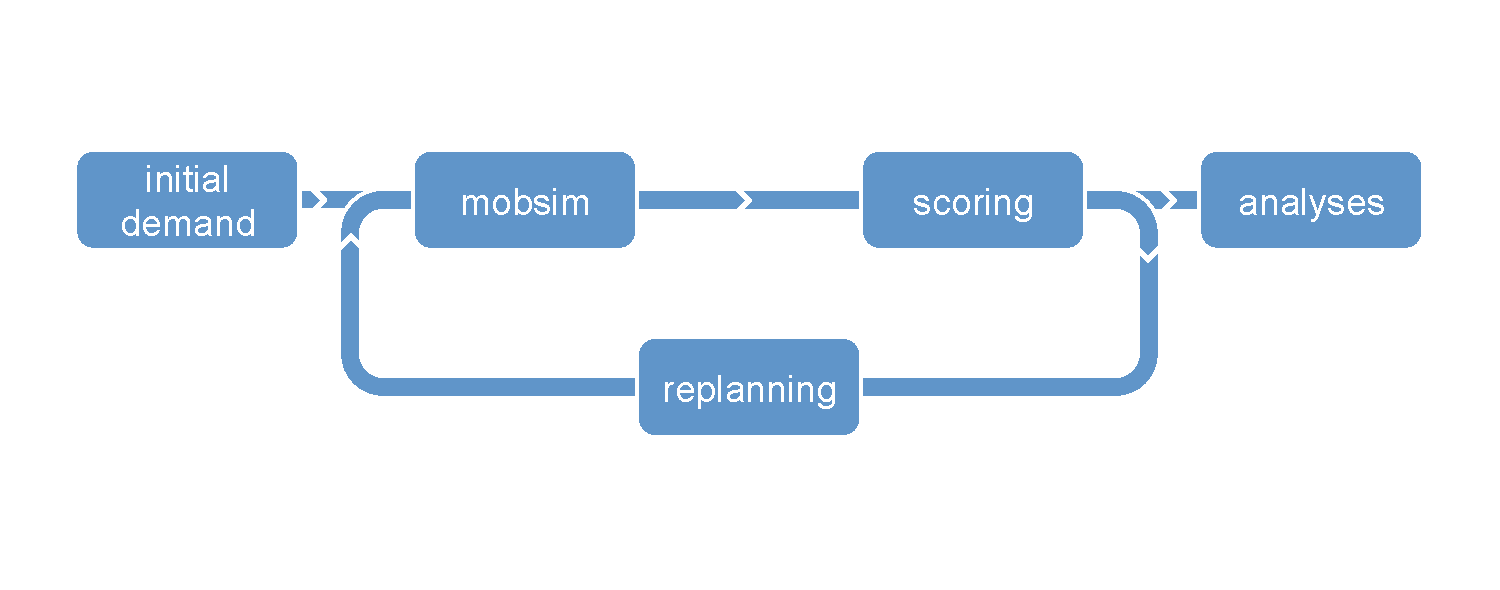
\includegraphics[width=0.8\textwidth]{figures/matsimcycle}

    \end{center}
  \end{titlepage}
  \cleardoublepage
}

%%%%%%%%%%%%%%%%%%%%%%%%%%%%%%%%%%%%%%%%%%%%%%%%%%%%%%%%%%%%%%%%%%%%%%

%%%%%%%%%%%%%%%%%%%%%%%%%%%%%%%%%%%%%%%%%%%%
%%%%%%%%%%%%%%%%%%%%%%%%%%%%%%%%%%%%%%%%%%%%
\newcommand{\createStandardInformationBasic}[4]{{\lstset{basicstyle=\normalsize\tt}%
%
\noindent\textbf{Entry point to documentation:}
\\
#1

\noindent\textbf{Invoking the module:}
\\
#2

%%\noindent\textbf{Configuration:}
%%\\
%%#3

\noindent\textbf{Selected publications:}
\\
#4
%
}}

%%%%%%%%%%%%%%%%%%%%%%%%%%%%%%%%%%%%%%%%%%%%
%%%%%%%%%%%%%%%%%%%%%%%%%%%%%%%%%%%%%%%%%%%%
% \ah{changed from extension to contribution, trying to be as specific is possible. This command so far is only used for contributions.}  

\newcommand{\entryStd}[1]{\url{http://matsim.org/extensions} $\to$ #1}

\newcommand{\invokeStd}[2]{\url{http://matsim.org/javadoc} $\to$ #1 $\to$ #2}

\newcommand{\invokeNonstd}[2]{No predefined invocation.  Starting point(s) under \url{http://matsim.org/javadoc} $\to$ #1 $\to$ #2.}

\newcommand{\configStd}[2]{\lstinline{#2} section(s) of the config file (only available when the #1 contribution is correctly loaded).}

\newcommand{\configNonstd}{Currently no config section available.}

\newcommand{\pubNone}{--}

\newcommand{\createStandardInformation}[4]{{\lstset{basicstyle=\normalsize\tt}%
%
\section{Basic Information}
\label{sec:#1-stdInfo}
%
\noindent\textbf{Entry point to documentation:}
\\
\entryStd{#1}

\noindent\textbf{Invoking the module:}
\\
\invokeStd{#1}{#2}

%%\noindent\textbf{Configuration:}
%%\\
%%\configStd{#1}{#3}
%
\noindent\textbf{Selected publications:}
\\
#4
%
}}

%%%%%%%%%%%%%%%%%%%%%%%%%%%%%%%%%%%%%%%%%%%%
%%%%%%%%%%%%%%%%%%%%%%%%%%%%%%%%%%%%%%%%%%%%%%%%%%%%%%%%%%%%%%%%%%%%%%
\definecolor{gray(x11gray)}{rgb}{0.75, 0.75, 0.75}
\definecolor{navyblue}{rgb}{0.0, 0.0, 0.5}
\definecolor{oceanboatblue}{rgb}{0.0, 0.47, 0.75}
\definecolor{steelblue}{rgb}{0.27, 0.51, 0.71}
\definecolor{lightgray}{rgb}{0.83, 0.83, 0.83}
\colorlet{shadecolor}{gray!20}

% removed background color: backgroundcolor=\color{shadecolor}

\usepackage{listings}
\lstset{%
%
backgroundcolor=\color{shadecolor},
%
language=Java,%
belowskip=-0pt,% ???
basicstyle=\ttfamily\lst@ifdisplaystyle\footnotesize\fi,%
lineskip=-0pt,% ???
keywordstyle=\lst@ifdisplaystyle\bfseries\color{blue}\fi,%
keywordstyle={[2]\lst@ifdisplaystyle\bfseries\color{magenta}\fi},%
commentstyle=\bfseries\lst@ifdisplaystyle\color{red}\fi,%
stringstyle=\bfseries\lst@ifdisplaystyle\color{ForestGreen}\fi,%
showstringspaces=false,%
frame=none,%
string=[b]",morekeywords={},morekeywords={[2]%
%
Comparator,String,
%
List,ArrayList,Map,TreeMap,HashMap,LinkedList,Set,Comparable,Collection,
%
% config and related:
Config,ConfigUtils,ConfigGroup,ReflectiveConfigGroup,
%
% scenario and related:
Id,Coord,Scenario,ScenarioUtils,
%
Population,Person,Plan,Activity,Leg,PlanElement,
%
Network,Link,Node,
%
Vehicle,
%
% controler and related:
Controler,EventsManager,StartupListener,StartupEvent,
%
% mobsim and related:
MobsimDriverPassengerAgent,PersonDriverAgentImpl,ActivityEngine,AgentSource,TeleportationEngine,
%
MobSim,QSim,MobsimAgent,DriverAgent,
%
TransitSchedule,
%
% important contribs (debatable if this should be highlighted):
RoadPricing,
%
DynAgent,DynAgentLogic,RandomDynLeg,RandomDynActivity,DynActivity,DynLeg,DriverDynLeg,PTPassengerDynLeg,PlanToDynAgentLogicAdapter,DynActivityEngine,DynAgentLauncherUtils,RandomDynActivity,RandomDynLeg,
%
}}

%I don't know why one needs a negative belowskip to get the space symmetric to the aboveskip.  Maybe this happens as long as one has parskip > 0?? kai, jan'15

\makeatletter
\lstnewenvironment{xml}{\lstset{%
%
backgroundcolor=\color{shadecolor},
%
%belowskip=-4pt,%
language=XML,basicstyle=\ttfamily\footnotesize,lineskip=-1pt,commentstyle=\bfseries\lst@ifdisplaystyle\color{red}\fi,stringstyle=\bfseries\lst@ifdisplaystyle\color{ForestGreen}\fi,showstringspaces=false,frame=none, string=[b]",morekeywords={[2]
%
description,
%
network,nodes,node,links,link,act,
%
networkChangeEvent,link,freespeed,
%
param,
%
population,person,plan,act,leg,route,
%
facilities,facility,activity,
%
vehicleDefinitions,vehicleType,vehicle,length,capacity,seats,standingRoom,
%
transitSchedule,
transitStops,stopFacility,
transitLine,transitRoute,transportMode,routeProfile,departures,departure,stop,
%
counts,count,volume,
%
config,module,param,parameterset,
%
roadpricing,cost,
%
},alsoletter={=}}}{}
%
% the "alsoletter={=}" seems to prevent that something like length="sldkfj"
% gets colored like an element
\makeatother

\makeatletter
\lstnewenvironment{shell}{\lstset{%
%
backgroundcolor=\color{shadecolor},
%
%belowskip=-4pt,%
language=bash,basicstyle=\ttfamily\footnotesize,lineskip=-1pt
%
}}
\makeatother

%%%%%%%%%%%%%%%%%%%%%%%%%%%%%%%%%%%%%%%%%%%%%%%%%%%%%%%%%%%%%%%%%%%%%%
\hyphenation{MATSim} % Word split: unknown words for latex. show how to split them.
\setcounter{tocdepth}{1}

\def\orange{\color{orange}}

%%%%%%%%%%%%%%%%%%%%%%%%%%%%%%%%%%%%%%%%%%%%%%%%%%%%%%%%%%%%%%%%%%%%%%
\newcommand{\mytitle}{The Multi-Agent Transport Simulation MATSim}
\newcommand{\myyear}{2015}
\newcommand{\karen}[1]{{\color{red} [\textbf{ke}: #1]}}
\newcommand{\ah}[1]{{\color{blue} [\textbf{ah}: #1]}}
\newcommand{\editdone}[1]{{\color{red} [\textbf{Edit done}: #1]}} \renewcommand{\editdone}[1]{\relax}
\newcommand{\kwaah}[1]{{\color{ForestGreen} [\textbf{kwa}: #1]}}
\newcommand{\gunnar}[1]{{\color{blue} [\textbf{gf}: #1]}}
\newcommand{\benjamin}[1]{{\color{red} [\textbf{bk}: #1]}}
\newcommand{\michaz}[1]{{\color{green} [\textbf{michaz}: #1]}}
\newcommand{\joschka}[1]{{\color{red} [\textbf{jb}: #1]}}
\newcommand{\kai}[1]{{\color{orange} [\textbf{kn}: #1]}}  % we still need \kai{} to make it compiling
\newcommand{\thibaut}[1]{{\color{BrickRed} [\textbf{td}: #1]}}
\newcommand{\dobi}[1]{{\color{blue} [\textbf{cd}: #1]}}
\newcommand{\marcel}[1]{{\color{BrickRed} [\textbf{mr}: #1]}}
\newcommand{\mm}[1]{\color{blue} [\textbf{mm}: #1] \color{black}}
\newcommand{\mnote}[1]{\medskip\centerline{{\sf\footnotesize\color{blue}\hfill #1}}\vspace{-.8em}}

\newcommand{\who}[1]{\color{red} \textit{[#1]} \color{black}}
%\newcommand{\todo}[1]{\color{ForestGreen} \textit{[TODO: #1]} \color{black}}
\newcommand{\copied}[1]{\color{ForestGreen} \textit{[copied: #1]} \color{black}}

%%\newcommand{\chkAtEnd}{{\color{gray} [check status before going to print]}}

\newcommand*{\eg}{e.g.,~}
\newcommand*{\ie}{i.e.,~}
\newcommand*{\cf}{cf.~}

% begin Gunnar: -----------------------------------
\ifxetex
%\usepackage{pstricks}
%\usepackage{pst-node}
%\usepackage{pstcol}
%\usepackage{pst-plot}
\fi

\newcommand{\MyEqRef}[1]{Equation~(\ref{#1})}
\newcommand{\note}[1]{\hl{[#1]}}
\newcommand{\Note}[1]{\note{#1}}
\renewcommand{\gunnar}[1]{\note{Gunnar: #1}}
\newcommand{\Gunnar}[1]{\gunnar{#1}}

%\newcommand{\corr}[2]{\st{#1} \ul{#2}}
\newcommand{\corr}[2]{#2}

\newtheorem{proposition}{Proposition}
\newtheorem{definition}{Definition}
\newcommand{\qedsymbol}{$\blacksquare$}
% end Gunnar: -----------------------------------

%%%%%%%%%%%%%%%%%%%%%%%%%%%%%%%%%%%%%%%%%%%%
%%%%%%%%%%%%%%%%%%%%%%%%%%%%%%%%%%%%%%%%%%%%
\usepackage{algorithm}
\makeatletter \renewcommand\thealgorithm{\thechapter.\arabic{algorithm}} \@addtoreset{algorithm}{chapter} \makeatother
%%%%%%%%%%%%%%%%%%%%%%%%%%%%%%%%%%%%%%%%%%%%
%%%%%%%%%%%%%%%%%%%%%%%%%%%%%%%%%%%%%%%%%%%%
%%\usepackage{ulem}
%%%%%%%%%%%%%%%%%%%%%%%%%%%%%%%%%%%%%%%%%%%%
%%%%%%%%%%%%%%%%%%%%%%%%%%%%%%%%%%%%%%%%%%%%
\def\vec#1{\boldsymbol{\mathbf{#1}}}
\def\imp#1{\textbf{#1}}
\def\eps{\varepsilon}
\def\matsimorg{\url{http://matsim.org}}
\def\javadoc{\url{http://matsim.org/javadoc}}
\def\extensions{\url{http://matsim.org/extensions}}
\def\faq{\url{http://matsim.org/faq}}
\def\issuetracker{\url{http://matsim.org/issuetracker}}
%%%%%%%%%%%%%%%%%%%%%%%%%%%%%%%%%%%%%%%%%%%%
%%%%%%%%%%%%%%%%%%%%%%%%%%%%%%%%%%%%%%%%%%%%%%%%%%%%%%%%%%%%%%%%%%%%%%
%% use hyper-refs for URL's and citations
\usepackage{hyperref}
\usepackage{bookmark}
%% line breaks for URL's
\usepackage{url}
\hypersetup{bookmarksdepth=3}
%%%%%%%%%%%%%%%%%%%%%%%%%%%%%%%%%%%%%%%%%%%%%%%%%%%%%%%%%%%%%%%%%%%%%%
%%%%%%%%%%%%%%%%%%%%%%%%%%%%%%%%%%%%%%%%%%%%
% inserting subpart level.  Related to subpart definition earlier, but as
% far as I can see it needs to be called fairly late or it is overwritten
% by something else (probably the hyperref package). kai, dec'15

\makeatletter
\def\toclevel@part{-2}
\def\toclevel@subpart{-1}
\makeatother

%%%%%%%%%%%%%%%%%%%%%%%%%%%%%%%%%%%%%%%%%%%%
%%%%%%%%%%%%%%%%%%%%%%%%%%%%%%%%%%%%%%%%%%%%%%%%%%%%%%%%%%%%%%%%%%%%%%
% When to use "newacronym" and "newglossaryentry"? 
% When used (referenced) for the first time both entries and accronyms are replaced by the short description in the text (not the one in [description={...}]). 
% For all further referencing only the name is shown.
% Accronyms, additionally show the abbreviation in brackets for the first time.

%##############################################################################################################################

\newacronym{api}{API}{Application Programming Interface}

\newacronym{aset}{ASET}{Available Safe Evacuation Time}

\newacronym[description={Assessment and Reliability of Transport Emission Models and Inventory Systems, a harmonized emission model in the \gls{eu}, possibly a predecessor of \gls{hbefa}, version 
3.1}]{artemis}{ARTEMIS}{Assessment and Reliability of Transport Emission Models and Inventory Systems}

\newacronym{bca}{BCA}{Benfit-Cost Analysis}

\newacronym[\glslongpluralkey={Battery Electric Vehicles}]{bev}{BEV}{Battery Electric Vehicle}

\newacronym[description={Berliner Verkehrsbetriebe (started as Berliner Verkehrs-Aktien-Gesellschaft)}]{bvg}{BVG}{Berliner Verkehrsbetriebe}

\newacronym[description={Calibration of Dynamic Traffic Simulations, see Chapter~\ref{ch:cadyts} and \citet{Floetteroed2010Manual110}}]{cadyts}{Cadyts}{Calibration of Dynamic Traffic Simulations}

\newacronym[\glslongpluralkey={Call Detail Records}]{cdr}{CDR}{Call Detail Record}

\newacronym[description={Comprehensive Econometric Microsimulator for Daily Activity-Travel Patterns \citep{BhatEtAl2008CEMDAPUserManual}}]{cemdap}{CEMDAP}{Comprehensive Econometric Microsimulator for Daily Activity-Travel Patterns}

\newacronym{cpu}{CPU}{Central Processing Unit}

\newacronym{create}{CREATE}{Campus for Excellence and Technological Enterprise}

\newacronym{cti}{CTI}{Commission for Technology and Innovation}

\newacronym{deqsim}{DEQSim}{Discrete Event Queue Simulation}

\newacronym{dfg}{DFG}{Deutsche Forschungsgemeinschaft}

\newacronym[description={District Métropolitain de Quito, Quito Metropolitan District}]{dmq}{DMQ}{Quito Metropolitan District}

\newacronym{drt}{DRT}{Demand Responsive Transport}

\newacronym{drv}{DRVs}{Disaster Response Vehicles}

\newacronym{dvrp}{DVRP}{Dynamic Vehicle Routing Problem}

\newacronym{ebptr}{EBPTR}{Events-Based Public Transport Router}

\newacronym[description={Enquesta de Mobilitat en dia Feiner, Barcelona’s annually transport survey}]{emef}{EMEF}{Enquesta de Mobilitat en dia Feiner}

\newacronym{emme}{EMME}{Equilibre Multimodal Multimodal Equilibrium} %\ah{check}

\newacronym{emme2}{EMME/2}{Equilibre Multimodal Multimodal Equilibrium/2} %\ah{check}

\newacronym[description={Emission Modeling Tool developed by \citet{HuelsmannEtAl_LAS_2011} and \citet{KickhoeferEtAl_VanoutriveVerhetsel_2013}}]{emt}{EMT}{Emission Modeling Tool}

\newacronym{emu}{EMU}{Expected Maximum Utility}

\newacronym{epsg}{EPSG}{European Petroleum Survey Group}

\newacronym{erp}{ERP}{Electronic Road Pricing}

\newacronym{eth}{ETH}{Eidgenössische Technische Hochschule}

\newacronym{esri}{ESRI}{Environmental Systems Research Institute}

\newacronym{eu}{EU}{European Union}

\newacronym[description={Evolutive User-centric Networks fOr Intraurban Accessibility \url{www.eunoia-project.eu}}]{eunoia}{EUNOIA}{Evolutive User-centric Networks fOr Intraurban Accessibility}

\newacronym{ev}{EV}{Electric Vehicle}

\newacronym{fcl}{FCL}{Future Cities Laboratory}

\newacronym[description={Forecasting Evolutionary Activity-Travel of Households and their Environmental RepercussionS \citep[][]{ArentzeEtAl_TRBTDF_2006}}]{feathers}{FEATHERS}{Forecasting Evolutionary Activity-Travel of Households and their Environmental RepercussionS}

\newacronym{fifo}{FIFO}{First In, First Out}

\newacronym{gb}{GB}{Giga Byte}

\newacronym{gdp}{GDP}{Gross Domestic Product}

\newacronym{gfip}{GFIP}{Gauteng Freeway Improvement Project}

\newacronym{gis}{GIS}{Geographic Information System}

\newacronym{gmbh}{GmbH}{Gesellschaft mit beschränkter Haftung}

\newacronym{gplv2}{GPLv2}{GNU General Public License version~2.0}

\newacronym{gps}{GPS}{Global Positioning System}

\newacronym{grips}{GRIPS}{GIS-based Risk-Analysis-, Information-, and Planning-System for Regional Evacuation}

\newacronym{gtha}{GTHA}{Greater Toronto and Hamilton Area}

\newacronym{gtfs}{GTFS}{General Transit Feed Specification}

\newacronym{gui}{GUI}{Graphical User Interface}

\newacronym{hafas}{HAFAS}{HaCon Fahrplan-Auskunfts-System}

\newacronym[description={Handbook on Emission Factors for Road Transport, version~3.1, see \url{www.hbefa.net}}]{hbefa}{HBEFA}{Handbook on Emission Factors for Road Transport}

\newacronym{hhtsd}{HHTSD}{Household Travel Survey Data}

\newacronym{hits}{HITS}{Household Interview Travel Survey}

\newacronym{ict}{ICT}{Information and Communications Technology}

\newacronym{ide}{IDE}{Integrated Development Environment}

\newacronym{ints}{INTS}{Irish National Travel Survey}

\newacronym{ipf}{IPF}{Iterative Proportional Fitting}

\newacronym{itsos}{ITSOS}{Intermodal Transport Simulation \& Operation System}

\newacronym{jar}{JAR}{Java ARchive}

\newacronym{javase}{Java SE}{Java Standard Edition}

\newacronym{jdeqsim}{JDEQSim}{Java Discrete Event Queue Simulation}

\newacronym[\glslongpluralkey={Key Performance Indicators}]{kpi}{KPI}{Key Performance Indicator}

\newacronym{kvmzh}{KVMZH}{Kantonales Verkehrsmodell Zürich}

\newacronym{lta}{LTA}{Singapore Land Transport Authority}

\newacronym{mb}{MB}{Mega Byte}

\newacronym{mfd}{MFD}{Macroscopic Fundamental Diagram}

\newacronym[description={Multi-Agent Transport Simulation, see \url{www.matsim.org}}, sort=matsim]{matsim}{\mbox{MATSim}}{Multi-Agent Transport Simulation}

\newacronym{mid}{MiD}{Mobilität in Deutschland}

\newacronym{mimosa}{MIMOSA}{Modélisation Isentrope du transport Méso-échelle de l'Ozone Stratosphérique par Advection}

\newacronym{mlipf}{MLIPF}{Multi-Level Iterative Proportional Fitting}

\newacronym{mnl}{MNL}{Multinomial Logit Model}

\newacronym{mobsim}{mobsim}{MATSim mobility simulation}

\newacronym[description={Motor Vehicle Emission Simulator, see \url{http://www.epa.gov/otaq/models/moves/}}]{moves}{MOVES}{Motor Vehicle Emission Simulator}

\newacronym{mpi}{MPI}{Message Passing Interface}

\newacronym{mrt}{MRT}{Mass Rapid Transit, Singapore}

\newacronym{msa}{MSA}{Method of Successive Averages}

\newacronym{nace}{NACE}{Nomenclature of Economic Activities}

\newacronym{nhts}{NHTS}{National Household Travel Survey}

\newacronym[description = {Nitrogen Dioxide}, name= {$\boldsymbol{NO_2}$}, sort={no2}]{no2}{$NO_2$}{Nitrogen Dioxide}

\newacronym[\glslongpluralkey={Norwegian Krones}]{nok}{NOK}{Norwegian Krone}

\newacronym{npts}{NPTS}{US Nationwide Personal Transportation Survey}

\newacronym{nybpm}{NYBPM}{New York Best Practice Model}

\newacronym{od}{O-D}{Origin-Destination}

\newacronym[description={OpenStreetMap \citep[][]{OpenStreetMap_Webpage_2015}}]{osm}{OSM}{OpenStreetMap}

\newacronym{phem}{PHEM}{Passenger car and Heavy-duty Emission Model}

\newacronym[\glslongpluralkey={Plugin Hybrid Electric Vehicles}]{phev}{PHEV}{Plugin Hybrid Electric Vehicle}

\newacronym[\glslongpluralkey={Points of Interest}]{poi}{POI}{Point of Interest}

\newacronym{powscar}{POWSCAR}{Place of Work, School or College Census of Anonymised Records}

\newacronym{psrc}{PSRC}{Puget Sound Regional Council}

\newacronym{pt}{PT}{Public Transit}

\newacronym[\glslongpluralkey={Public Transit Operators}]{pto}{PTO}{Public Transit Operator}

\newacronym{ram}{RAM}{Random Access Memory}

\newacronym{rset}{RSET}{Required Safe Egress Time}

\newacronym{rum}{RUM}{Random Utility Model}

\newacronym[description={Simulation and Assignment of Traffic to Urban Road Networks \citep{SATURN_Webpage_2014}}]{saturn}{SATURN}{Simulation and Assignment of Traffic to Urban Road Networks}

\newacronym{sanral}{SANRAL}{South African National Roads Agency Limited}

\newacronym{sbptr}{SBPTR}{Schedule-Based Public Transport Router}

\newacronym{sec}{SEC}{Singapore-ETH Centre for Global Environmental Sustainability}

\newacronym{sma}{SMA}{Seoul Metropolitan Area}

\newacronym{snf}{SNF}{Schweizerischer Nationalfonds}

\newacronym{spi}{SPI}{Service Provider Interface}

\newacronym{spss}{SPSS}{Statistical Package for the Social Sciences}

\newacronym{soc}{SOC}{State of Charge}

\newacronym{srv}{SrV}{System repräsentativer Verkehrserhebungen, Berlin}

\newacronym{sue}{SUE}{Stochastic User Equilibrium}

\newacronym[description={A project addressing the modeling and computational issues of integrating modern mobility simulations with the latest micro-simulation land use models, see \url{http:\\www.sustaincity.org}}]{sustaincity} {SustainCity}{Using land use models for sustainable policy making}

\newacronym{svn}{SVN}{Apache SubVersioN}

\newacronym{tasha}{TASHA}{Travel Activity Scheduler for Household Agents}

\newacronym[\glslongpluralkey={Traffic Analysis Zones}]{taz}{TAZ}{Traffic Analysis Zone}

\newacronym{tesf}{TESF}{Transportation Energy Simulation Framework}

\newacronym{transcad}{TransCAD}{Transportation Computer Assisted Design}

\newacronym{transims}{TRANSIMS}{TRansportation ANalysis and SIMulation System}

\newacronym{tts}{TTS}{Transportation Tomorrow Survey}

\newacronym[description={Software-based simulation system for supporting planning and analysis of urban development, see \url{http:\\www.urbansim.org}.}]{urbansim}{UrbanSim}{Tool for simulation of urban development}

\newacronym{utm}{UTM}{Universal Transverse Mercator}

\newacronym{uvek}{UVEK}{Eidgenössisches Departement für Umwelt, Verkehr, Energie und Kommunikation}

\newacronym{v2g}{V2G}{Vehicle-to-Grid}

\newacronym[description={Verkehr In St\"adten \textendash\ SImulationsModell, see \url{www.ptv.de}}]{vissim}{VISSIM}{Verkehr In St\"adten \textendash\ SImulationsModell}

\newacronym[description={Verkehr In St\"adten \textendash\ UMlegung, see \url{www.ptv.de}}]{visum}{VISUM}{Verkehr In St\"adten \textendash\ UMlegung}

\newacronym{vrp}{VRP}{Vehicle Routing Problem}

\newacronym{vtts}{VTTS}{Value of Travel Time Savings}

\newacronym{wkt}{WKT}{Well-Known Text}

\newacronym[description={Extensible Markup Language, see \url{www.w3.org/XML/}}]{xml}{XML}{Extensible Markup Language}

\newacronym[description={XRef: Cross References documentation, for \gls{matsim} see \url{http://matsim.org/xref}}]{xref}{XRef}{Cross References}

% ##############################################################################################################################

%%%%%%%%%%%%%%%%%%%%%%%%%%%%%%%%%%%%%%%%%%%%
%%%%%%%%%%%%%%%%%%%%%%%%%%%%%%%%%%%%%%%%%%%%
% Wann benutzt man "newacronym", wann "newglossaryentry"? ##############################################################################################################################

% bk ========================================================================
\newacronym[description={Assessment and Reliability of Transport Emission 
Models and Inventory Systems, a harmonized emission model in the \acrlong{eu}, 
possibly a predecessor of \acrshort{hbefa}, version 
3.1}]{artemis}{ARTEMIS}{Assessment and Reliability of Transport Emission Models 
and Inventory Systems}

\newacronym[description={The Emission Modeling Tool developed by \citet{HuelsmannEtAl_LAS_2011} and \citet{KickhoeferEtAl_VanoutriveVerhetsel_2013}}]{emt}{EMT}{Emission Modeling Tool}

\newacronym{eu}{EU}{European Union}

\newacronym[description={Handbook on Emission Factors for Road Transport, 
version 3.1, see \url{www.hbefa.net}}]{hbefa}{HBEFA}{Handbook on Emission 
Factors for Road Transport}

\newacronym[description={Multi-Agent Transport Simulation, see 
\url{www.matsim.org}}, sort=matsim]{matsim}{\mbox{MATSim}}{Multi-Agent 
Transport Simulation}

\newacronym{mimosa}{MIMOSA}{A macroscopic emission model}

\newacronym[description={Motor Vehicle Emission Simulator, 
see \url{http://www.epa.gov/otaq/models/moves/}}]{moves}{MOVES}{Motor Vehicle 
Emission Simulator}

\newacronym[description={Nitrogen Dioxide}, %sort={no2},
nonumberlist]{no2}{\ensuremath{\mathit{NO_2}}}{Nitrogen Dioxide}

\newacronym{phem}{PHEM}{Passenger car and Heavy-duty Emission Model}

\newacronym{pt}{PT}{public transit}

\newacronym[description={Verkehr In St\"adten \textendash\ SImulationsModell, 
see \url{www.ptv.de}}]{vissim}{VISSIM}{Verkehr In St\"adten \textendash\ 
SImulationsModell}

\newacronym[description={Verkehr In St\"adten \textendash\ UMlegung, 
see \url{www.ptv.de}}]{visum}{VISUM}{Verkehr In St\"adten \textendash\ UMlegung}

\newacronym[description={Extensible Markup Language, see 
\url{www.w3.org/XML/}}]{xml}{XML}{Extensible Markup Language}

% bk ========================================================================

\newglossaryentry{mnl}
{
    name=MNL,
    description={Multinomial Logit Model ...}
}

\newglossaryentry{java}
{
    name=JAVA,
    description={programming language ...}
}

\newglossaryentry{mobsim}
{
    name=mobsim,
    description={MATSim mobility simulation ...}
}


%day plan = schedule
%
%contribution = MATSim extensions (do not use extension as a name anymore?)
%
%transit
% ##############################################################################################################################

